\subsection{Use Case 5: Request Verification}

\subsubsection{General Description}
\begin{tabular}{|p{.2\linewidth}|p{.65\linewidth}|}
\hline 
ID: & Request Verification \\ \hline
Goal: & Get a verified account. \\ \hline
Precondition: & The user must be logged in with an advertiser account.  \\ \hline
Postcondition: & The advertiser can now be approved. \\ \hline
Involved Users: & Advertiser: Portrays doctors, medical companies and so forth, who use the system to place advertisements. \\ \hline
\end{tabular}

\subsubsection{UI to call the use case}
\begin{minipage}{1\textwidth}
\begin{figure}[H]
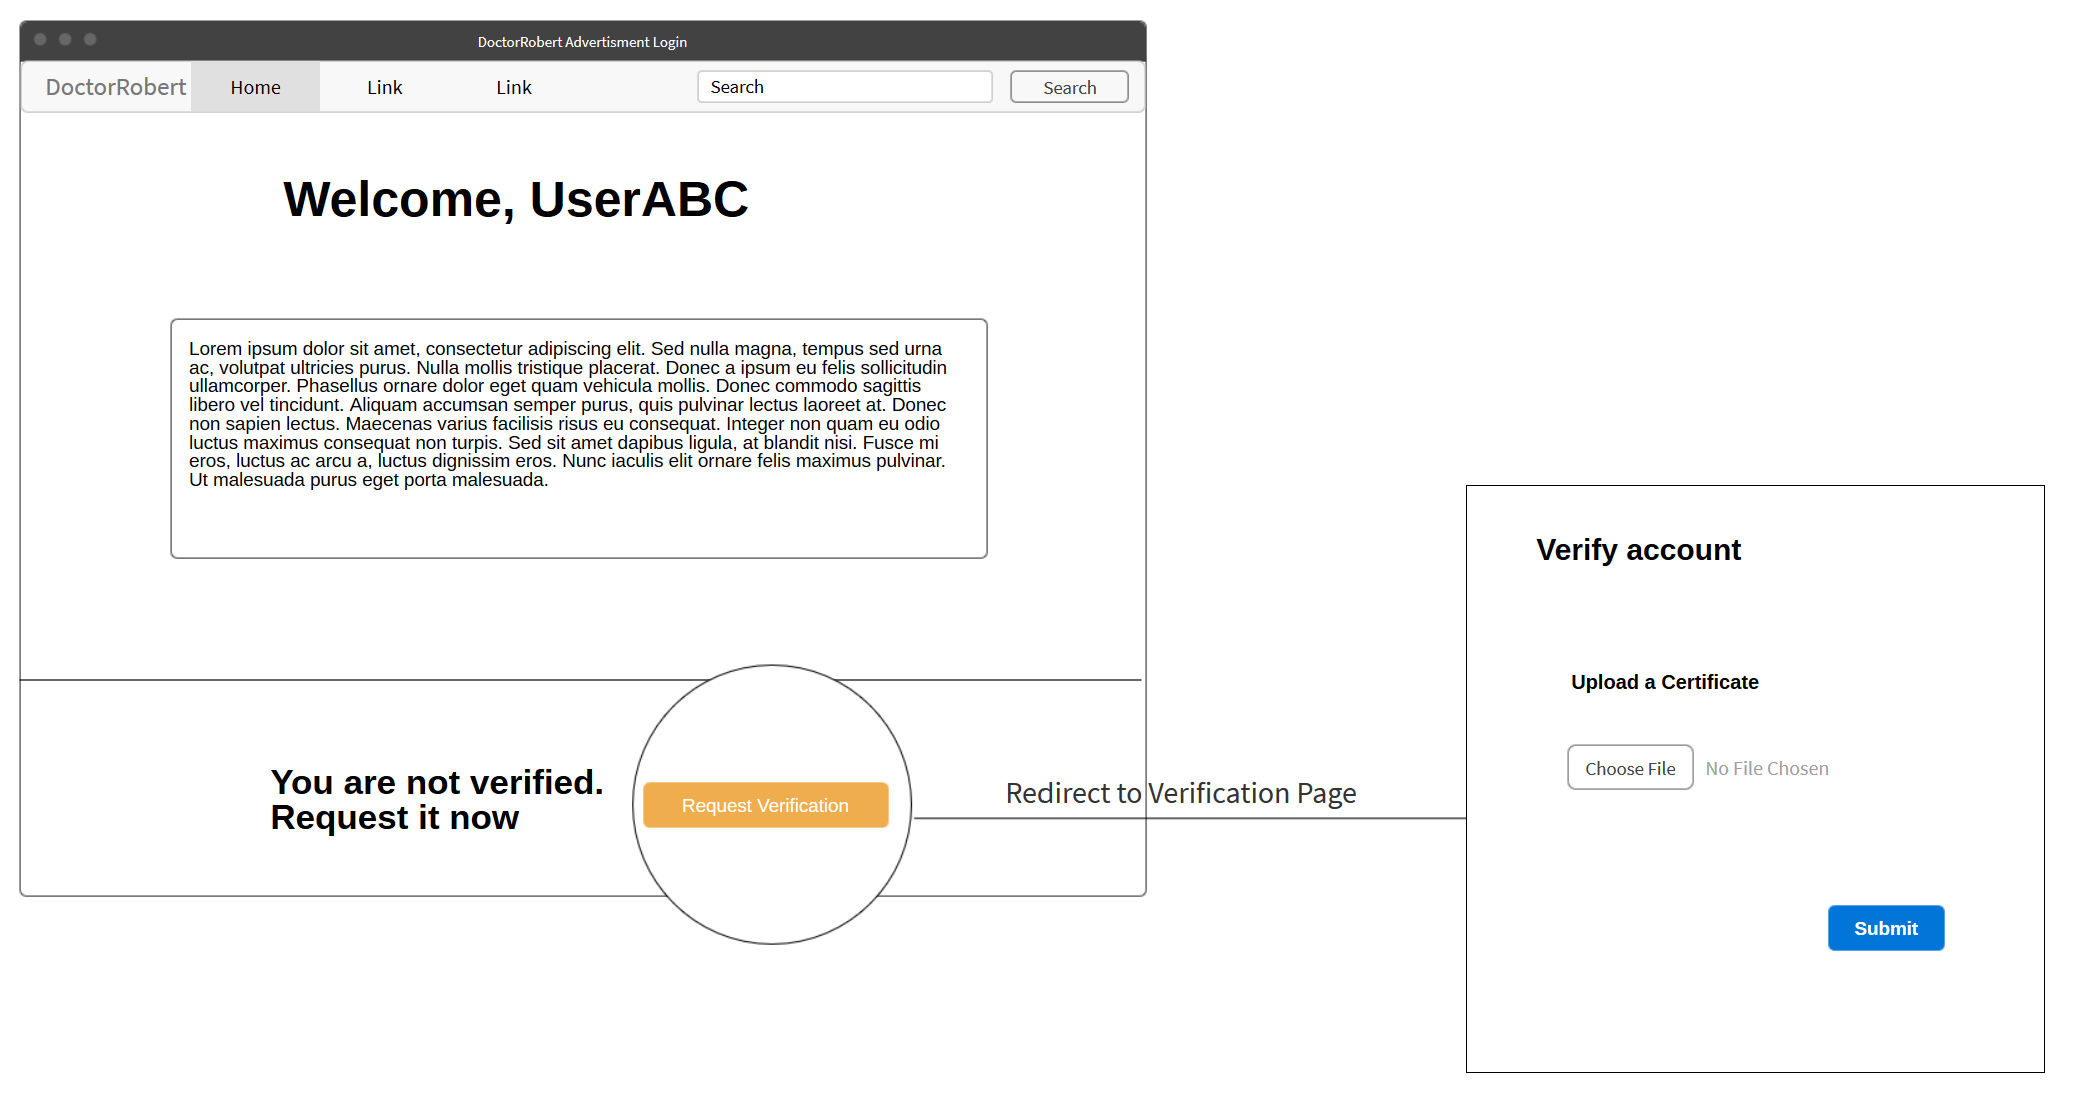
\includegraphics[scale=.65]{SystemSpec/Usecases/Mocks/reqVeri01.png}\\
\caption{\label{fig:blue_rectangle}Request Verification UI}
\end{figure}
\end{minipage} \hfill
\begin{minipage}{1\textwidth}
The advertisement portal will only be available as web application since there is no need for an ordinary customer to access it via the mobile app.
The main screen of an advertiser account gives the option to request verification for this advertiser, by pressing the responsible button, if not already verified. After pressing the "Request Verification"-Button the advertiser has to select two files, one containing some sort of certificate and the second an possible way of identification. For instance a personalized picture containing the contenders face an ID and a handwritten message with a randomly generated message on it.
In the end the files will be sent to us for verification.
\end{minipage}

\subsubsection{The Standard Use}

\begin{minipage}{0.5\textwidth}
\begin{figure}[H]
\centering
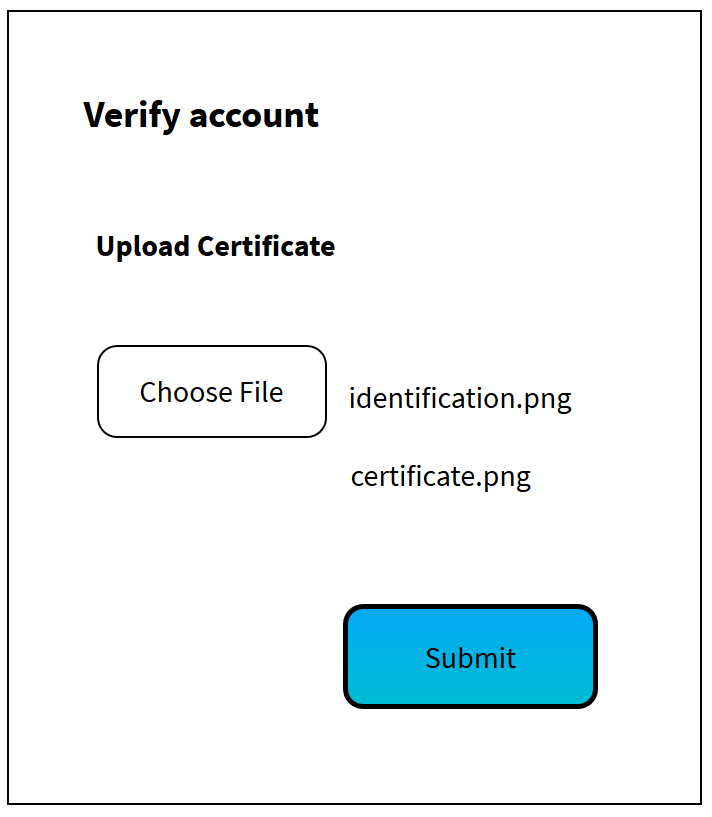
\includegraphics[scale=.8]{SystemSpec/Usecases/Mocks/reqVerNormal.png}\\
\caption{\label{fig:blue_rectangle}Standard Use}
\end{figure}
\end{minipage} \hfill
\begin{minipage}{0.5\textwidth}
The advertiser chooses to upload .png-Files containing a certificate and identification, then submits these for verification.
\end{minipage}

\begin{center}
\begin{figure}[H]
\centering
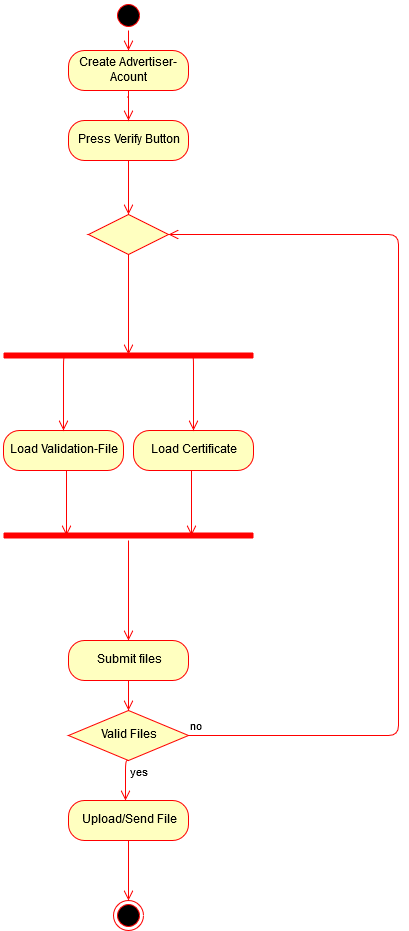
\includegraphics[scale=0.5]{SystemSpec/Usecases/Diagrams/RequestVerificationActivity.png}
\caption{\label{fig:blue_rectangle}Request Verification Activity}
\end{figure}
\end{center}

\subsubsection{The Non-Standard Use}

\begin{minipage}{0.5\textwidth}
\begin{figure}[H]
\centering
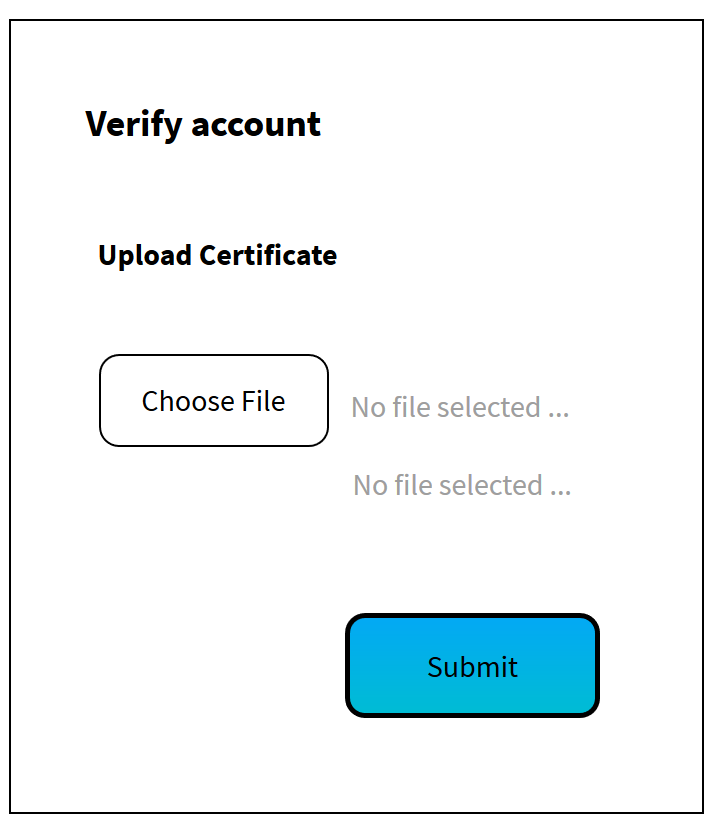
\includegraphics[scale=.6]{SystemSpec/Usecases/Mocks/reqVerNon02.png}\\
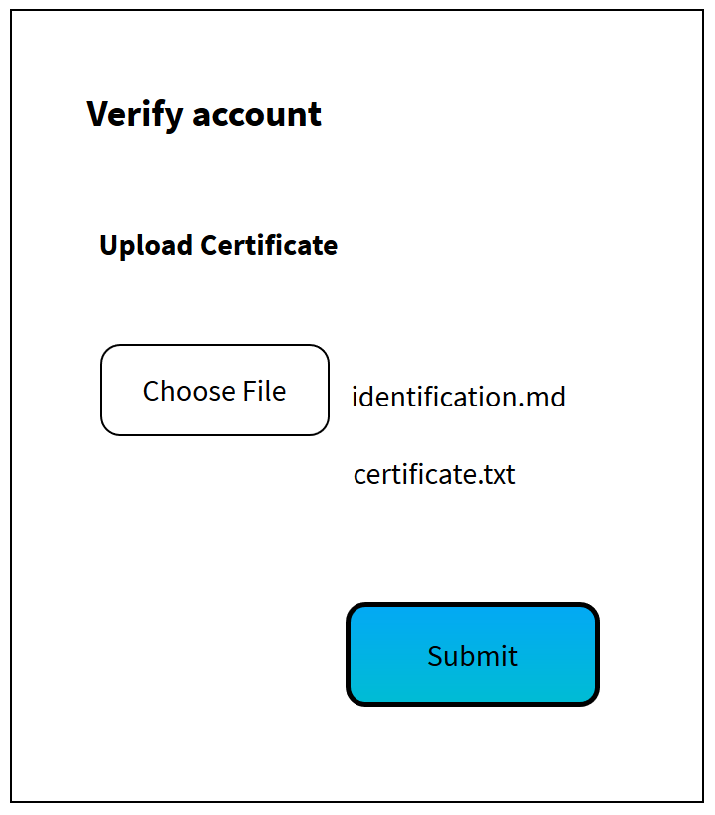
\includegraphics[scale=.6]{SystemSpec/Usecases/Mocks/reqVerNon01.png}\\
\caption{\label{fig:blue_rectangle}Non-Standard Uses}
\end{figure}
\end{minipage} \hfill
\begin{minipage}{0.5\textwidth}
The types of the uploaded files are either of a wrong format, blank empty Files or the advertiser did not select files at all. 
\end{minipage}

\pagebreak
